

%figurstørrelser.

\documentclass[reprint,english,notitlepage]{revtex4-1}  % defines the basic parameters of the document
% if you want a single-column, remove reprint

% allows special characters (including æøå)
\usepackage[utf8]{inputenc}
\usepackage [norsk]{babel} %if you write norwegian
%\usepackage[english]{babel}  %if you write english


%% note that you may need to download some of these packages manually, it depends on your setup.
%% I recommend downloading TeXMaker, because it includes a large library of the most common packages.

\usepackage{physics,amssymb}  % mathematical symbols (physics imports amsmath)
\usepackage{graphicx}         % include graphics such as plots
\usepackage{xcolor}           % set colors
\usepackage{hyperref}         % automagic cross-referencing (this is GODLIKE)
\usepackage{tikz}             % draw figures manually
\usepackage{listings}         % display code
\usepackage{subfigure}        % imports a lot of cool and useful figure commands

% defines the color of hyperref objects
% Blending two colors:  blue!80!black  =  80% blue and 20% black
\hypersetup{ % this is just my personal choice, feel free to change things
    colorlinks,
    linkcolor={red!50!black},
    citecolor={blue!50!black},
    urlcolor={blue!80!black}}

%% Defines the style of the programming listing
%% This is actually my personal template, go ahead and change stuff if you want
\lstset{ %
	inputpath=,
	backgroundcolor=\color{white!88!black},
	basicstyle={\ttfamily\scriptsize},
	commentstyle=\color{magenta},
	language=Python,
	morekeywords={True,False},
	tabsize=4,
	stringstyle=\color{green!55!black},
	frame=single,
	keywordstyle=\color{blue},
	showstringspaces=false,
	columns=fullflexible,
	keepspaces=true}

%% USEFUL LINKS:
%%
%%   UiO LaTeX guides:        https://www.mn.uio.no/ifi/tjenester/it/hjelp/latex/
%%   mathematics:             https://en.wikibooks.org/wiki/LaTeX/Mathematics

%%   PHYSICS !                https://mirror.hmc.edu/ctan/macros/latex/contrib/physics/physics.pdf

%%   the basics of Tikz:       https://en.wikibooks.org/wiki/LaTeX/PGF/TikZ
%%   all the colors!:          https://en.wikibooks.org/wiki/LaTeX/Colors
%%   how to draw tables:       https://en.wikibooks.org/wiki/LaTeX/Tables
%%   code listing styles:      https://en.wikibooks.org/wiki/LaTeX/Source_Code_Listings
%%   \includegraphics          https://en.wikibooks.org/wiki/LaTeX/Importing_Graphics
%%   learn more about figures  https://en.wikibooks.org/wiki/LaTeX/Floats,_Figures_and_Captions
%%   automagic bibliography:   https://en.wikibooks.org/wiki/LaTeX/Bibliography_Management  (this one is kinda difficult the first time)
%%   REVTeX Guide:             http://www.physics.csbsju.edu/370/papers/Journal_Style_Manuals/auguide4-1.pdf
%%
%%   (this document is of class "revtex4-1", the REVTeX Guide explains how the class works)


%% CREATING THE .pdf FILE USING LINUX IN THE TERMINAL
%%
%% [terminal]$ pdflatex template.tex
%%
%% Run the command twice, always.
%% If you want to use \footnote, you need to run these commands (IN THIS SPECIFIC ORDER)
%%
%% [terminal]$ pdflatex template.tex
%% [terminal]$ bibtex template
%% [terminal]$ pdflatex template.tex
%% [terminal]$ pdflatex template.tex
%%
%% Don't ask me why, I don't know.

\begin{document}



\title{Oppgave 1A.6: En forenklet kode for en rakettmotor}
\date{\today}
\author{Knadidatnr.: 15889}
\affiliation{Institute of Theoretical Astrophysics, University of Oslo}
\email{textme@astro.uio.no}


\newpage

\begin{abstract}
Jeg har laget en forenklet simulering av en rakettmotor. Målet med prosjektet er å finne
 ut hva som skal til for å løfte en satelitt på 1000kg fra overflaten av planeten Bayport.
 Planeten har en masse på $1.38865*10^{25}$kg, det er 2.33 så mye som massen til jorda.
 Radien til planeten er 8 376km, 1.31 ganger så stor som radien til jorda.
\end{abstract}
\maketitle                                % creates the title, author, date & abstract



\section{Introduksjon}
\label{sect:intro}

I et fjernt solsystem med 7 planeter og en hvitglødende stjerne bor det en gruppe
 skapninger som ikke har kommet like langt i den teknologiske utviklingen som vi mennesker
 har gjort her på jorda. Deres samfunn er bygget på hardt fysisk arbeid, og de har et
 sterkt behov for slappe av. De har selvfølgelig hørt om menneskehetens største bragd;
 oppfinnelsen av fjernsynsapparatet. Med litt hjelp har de bygget en satelitt som kan
 forsyne innbyggerne av planeten med TV-signaler fra rommet. Men for at de skal få nytte
 av satelitten må den skytes opp i bane rundt planeten. Dette skal vi hjelpe dem med!

Planeten har en unnslipningshastighet på 14,9km/s. Jordas, til sammenlikning, er 11,2km/s.
 Vi må akselerere satelitten, som harmasse 1000kg, til denne farten for at den skal kunne
 unnslippe gravitasjonskraften til planeten. Vi skal derfor gjøre en simulasjon av en
 rakettmotor for å finne ut hvor stor motor og hvor mye drivstoff vi trenger for å kunne
 sende raketten med TV-satelitten vår ut i verdensrommet.

Prinsippet bak rakettmotoren er i utganspunktet veldig enkelt. Jeg skal forklare
 nødvendige detaljer her, for en mer omfattende beskrivelse, se \citep{part1A}. Nederst i
 raketten har vi et kammer med varm hydrogengass. Avhengig av temperaturen i gassen vil
 disse gassmolekylene bevege seg med forskjellige middelhastigheter, og dermed kollidere
 med veggene med ulik kraft mellom vegg og molekyl. Dersom vi har et hull i bunnen av
 kammeret vårt vil gassmolekylene etter hvert slippe ut her. Siden bevegelsesmengden til
 systemet som består av raketten og gassmolekylene skal være bevart (mer om dette i metode-
 seksjonen) vil raketten få en positiv akselerasjon i motsatt retning av det de unnslupne
 gasspartiklene beveger seg. Dette er det fysiske prinsippet vi baserer oss på for å få
 satelitten i bane rundt planeten vår!

Det melder seg umiddelbart noen problemer når vi forsøker å modellere dette, først og
 fremst kapasiteten til datamaskinen vi bruker til å utføre beregningene. Dersom vi ser
 bort fra gravitasjonskraften under akselerasjonen og lar være å tenke på at massen til
 drivstoffet vi må bære med oss også skal akselereres, finner vi likevel ved å betrakte
 bevaring av bevegelsesmengde at vi må ha med oss over 1000kg hydrogengass. Dette
 tilsvarer ca. $3*10^{29}$ partikler dersom vi antar at alle molekylene i gassen er H$_2$O-
 molekyler. Skal man modellere prosessen i detalj må vi egentlig følge alle disse
 gassmolekylene. Dette lar seg ikke gjøre, det ville blitt altfor mange beregninger å
 utføre. Det vi i stedet kan gjøre er å dele kammeret inn i mange små bokser som hver bare
 inneholder en liten andel av det totale antall gassmolekyler. Det viser seg at ved å
 gange opp resultatene vi da får med antall bokser vi deler kammeret inn i, kan vi komme
 nært de observasjonene vi gjør i virkeligheten\citep{part1A}. På denne måten kan vi
 simulere systemet. Vi kommer også til å kunne sammelikne resultatene med det vi forventer
 å finne ut fra analytiske beregninger, og regner med at disse kommer til å ligge svært
 nær hverandre.


\section{Metode}

Alle analytiske uttrykk i denne seksjonen bygger på utledninger som kan finnes i
 \citep{part1A}. Vi betrakter en kubisk boks med sidekanter av lengde $L = 10^{-6}$m. I denne boksen følger vi bevegelsene til $N = 10^5$ hydrogengassmolekyler, og vi setter absolutt temperatur til å være 10 000K. Vi kan med god tilnærming betrakte innholdet i boksen som en ideell gass. Det betyr at alle kollisjoner er elastiske og at vi ser på alle partiklene som punktpartikler. Vi ser bort fra all interaksjon mellom partiklene, det eneste som endrer bevegelsen til gasspartiklene er når de kolliderer elastisk med veggene i boksen. Når de kolliderer med veggen, er det bare hastighetskomponenten som står normalt på veggen som endres fordi det ikke virker noen krefter i de to retningene som ggår langs veggen.

\begin{figure}[htbp]
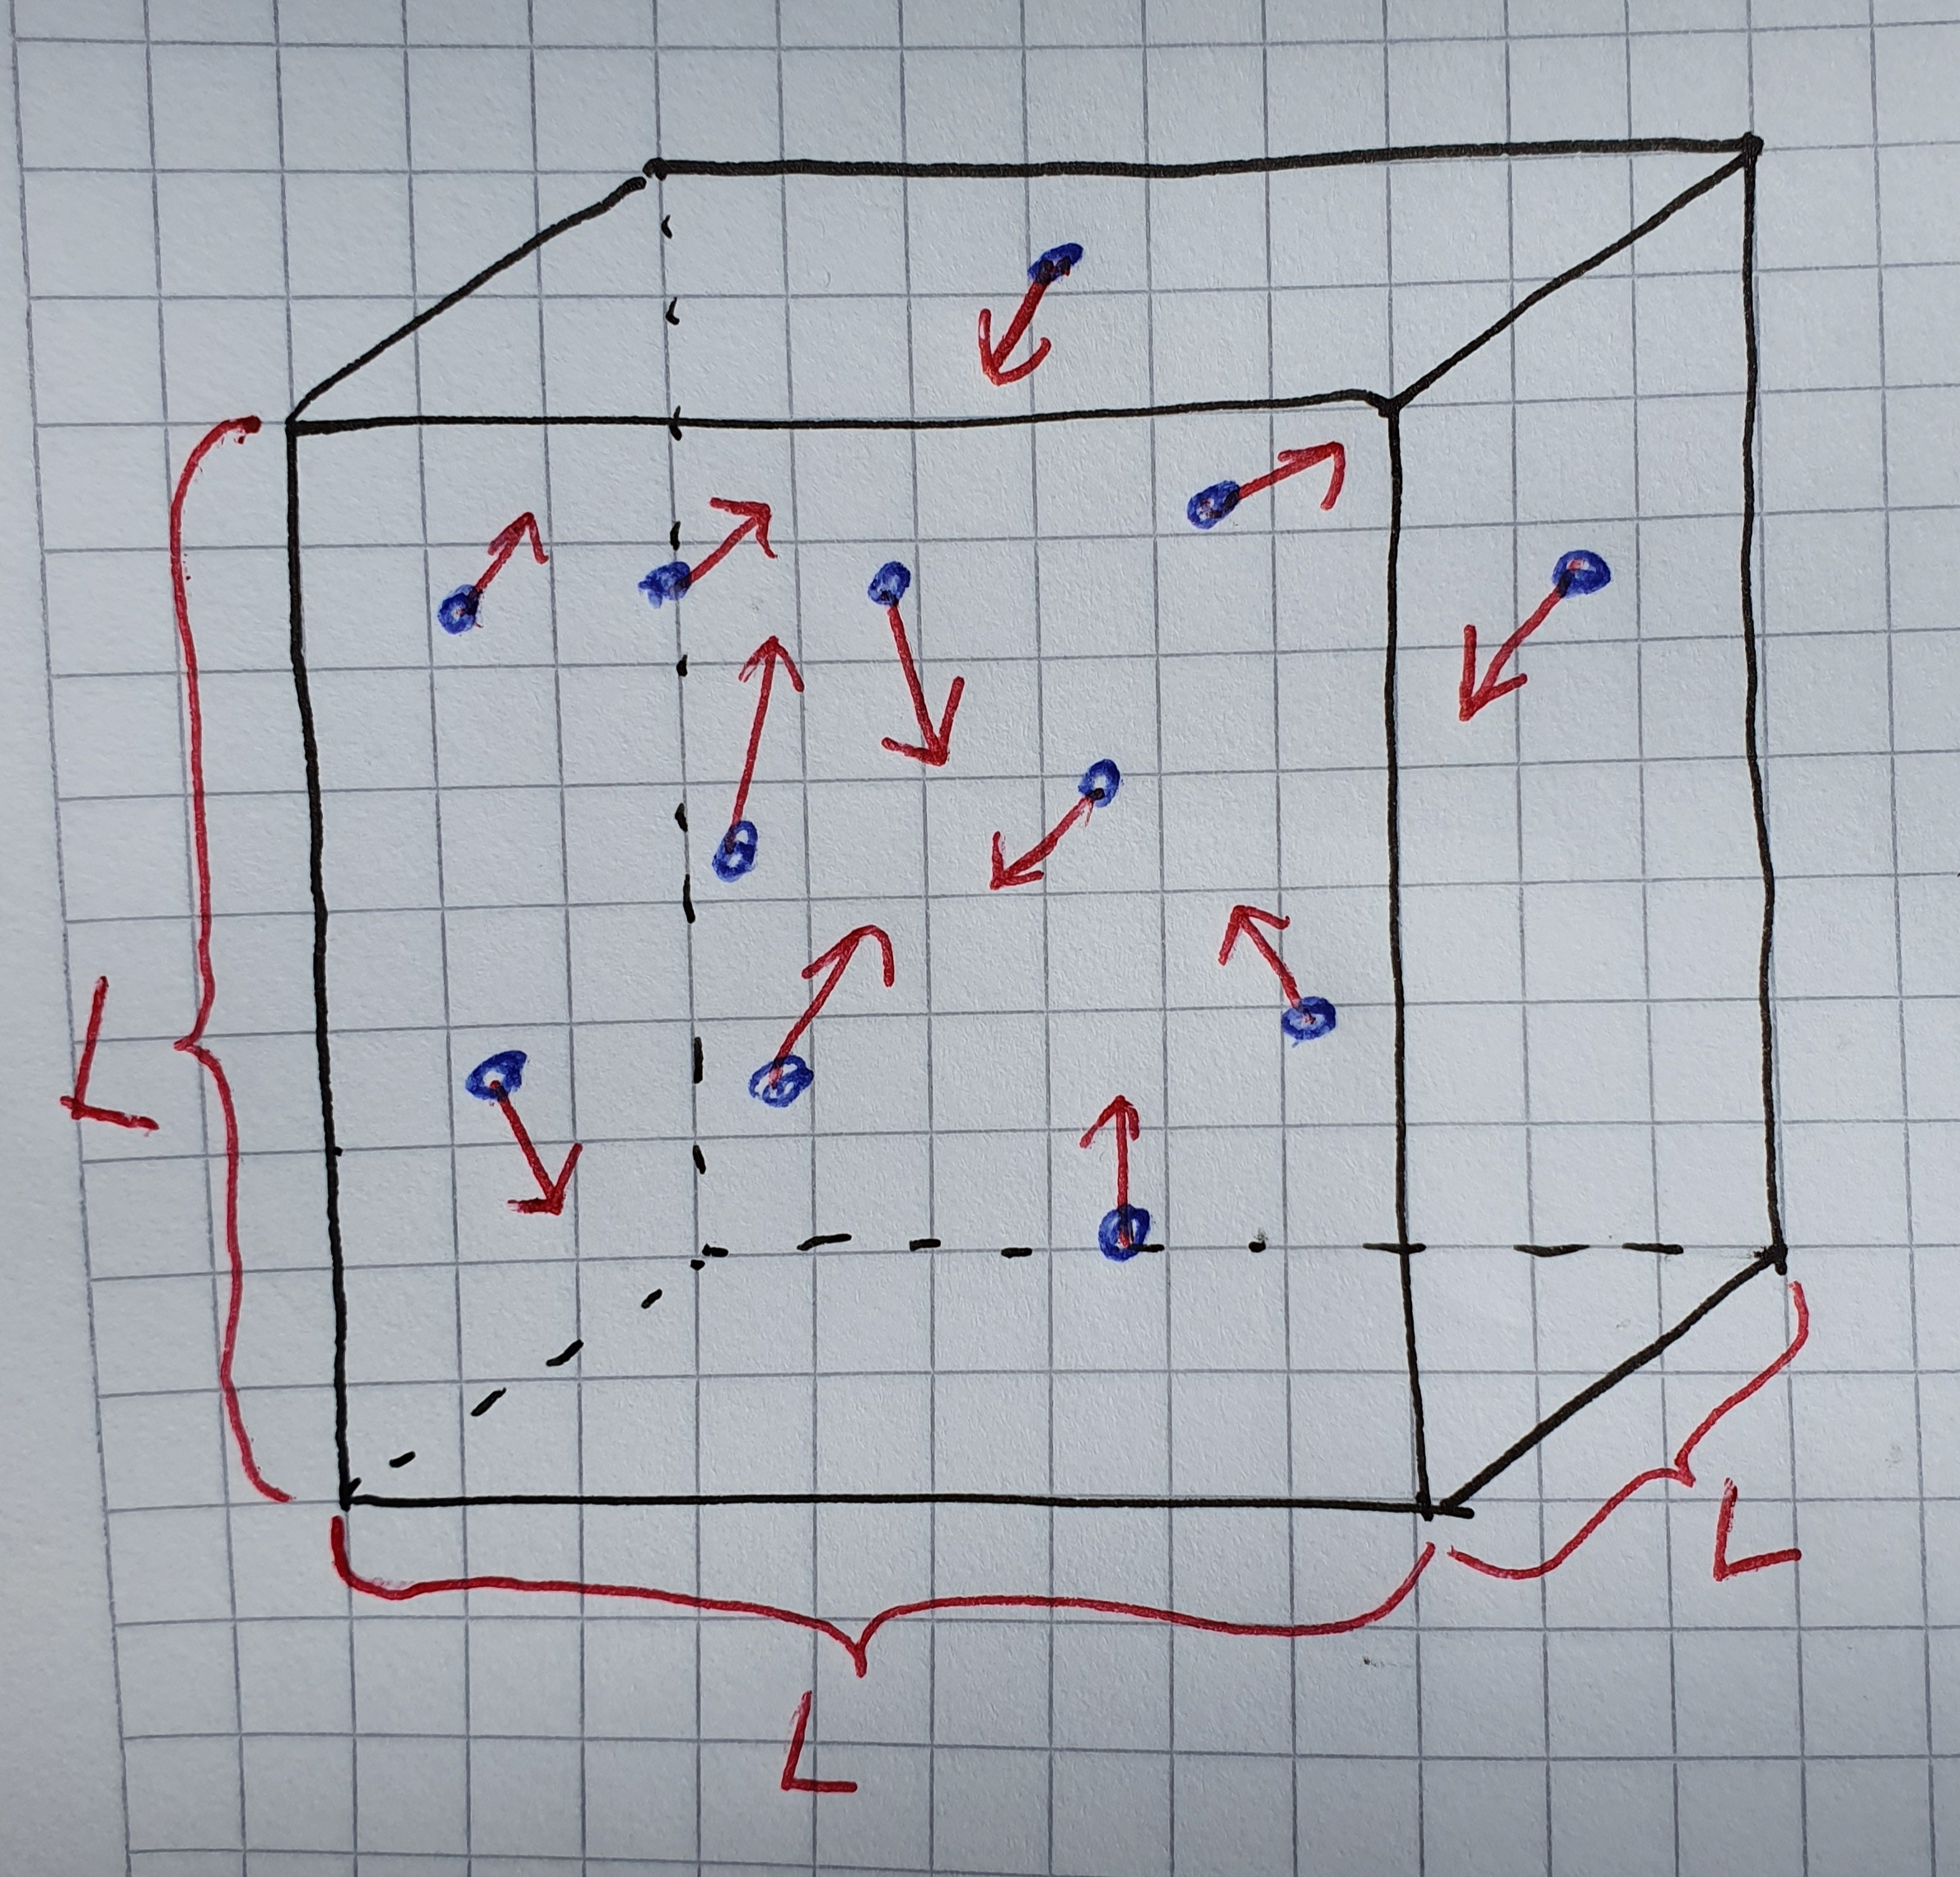
\includegraphics[width=0.5\linewidth]{boks.jpg}
\caption{Figuren viser boksen med noen av gasspartiklene tegnet inn. Pilene viser retningen og størrelsen til hastighetene.\label{fig:boks}}
\end{figure}

Vi starter med å fordele alle gasspartiklene rundt i boksen, hver med en initialhastighet
 $\vec{v}_0$. Vi regner med at gassen er uniformt fordelt i boksen, det vil si at sannsynligheten for å finne en gasspartikkel på ett bestemt sted i boksen er like stor for alle punkter i hele boksen. Hastighetene i er normalfordelt i hver retning, med middelverdi 0 og standardavvik
 \[
 \sigma = \sqrt{\frac{kT}{m}}
 \]
 der $k$ er Boltzmannkonstanten, $T$ er absolutt temperatur til gassen og $m$ er massen til et hydrogengassmolekyl i kg. Vi dobbelsjekker initialiseringen ved å løpe over alle partiklene og sjekke den midlere farten og kinetiske energien til partiklene i gassen mot analytiske uttrykk. Den gjennomsnittlige kinetiske energien til molekylene i gassen er gitt ved
 \begin{equation}
 \label{eq:kinetic}
 K = \frac{3}{2}kT
 \end{equation}
 der $K$ er kinetisk energi og $k$ og $T$ igjen er Boltzmannkonstanten og absolutt temperatur.

Ved å lage en algoritme som styrer bevegelsen til partiklene inne i boksen (det eneste den
 skal gjøre er å snu partiklene når de treffer veggene), kan vi nå simulere situasjonen i boksen. Jeg har laget en buffersone på 0.0125L på begge sider av alle veggene slik at alle partikler som er innenfor dette området og på vei ut vil bli snudd. Målet med dette var at noen partikler ville bli snudd like før de treffer veggen i boksen, mens noen blir snudd like etter. Siden vi beregner bevegelsene til partiklene i fiksede tidspunkter, er det umulig å snu alle partiklene akkurat idet de treffer veggen siden dette alltid vil skje mellom to tidssteg. Ved å snu noen partikler før de har gått gjennom veggen og andre partikler etter at de har gått gjennom veggen vil volumet til boksen i simuleringen komme så nært som mulig det volumet vi skal ha. Dette vil for eksempel være avgjørende for å beregne trykket.

Ved å registrere bevegelsesmengden til partiklene som kolliderer med veggene, kan vi regne
 ut det simulerte trykket og igjen sammenlikne dette med det analytiske uttrykket for trykket i gassen. Dette analytiske uttrykket for trykket er kjent som idealgassloven:
 \[
 P = nkT
 \]
 der $n$ er antall partikler per volum, $k$ er Boltzmannkonstanten og $T$ er absolutt temperatur. For å finne trykket i simuleringen når vi kjenner bevegelsesmengden til partiklene som kolliderer med den ene veggen må vi gjøre litt mer regning. Ettersom den kinetiske energien skal være bevart under kollisjonen må absoluttverdien av bevegelsesmengden til partikkelen være den samme etter støtet som før. Det er bare farten i retningen som står vinkelrett på veggen som endrer seg, la oss nå si at det er farten i x-retning, $v_x$). Da må vi ha at $v_x = - v_{0, x}$ slik at absoluttverdien av hastigheten er den samme før og etter støtet, men etter støtet er partikkelen på vei bort fra veggen. Da får vi at endringen av bevegelsesmengde er $2 p_x$. Kraften utøvd på veggen i løpet av et tidsintervall $\Delta t$ er i henhold til Newton's andre lov

\begin{equation}
  \label{eq:p_force}
  f = \frac{2 p_x}{\Delta t}
\end{equation}
 se \citep{part1A}. Hvis vi da registrerer $p_x$ til alle partiklene som kolliderer med én vegg i løpet av simulasjonen kan vi finne det samlede trykket ved å dele på varigheten av simulasjonen. Trykk er definert ved

 \begin{equation}
   \label{eq:pressure}
   P = F/A
 \end{equation}
 der P er trykket, F er den samlede kraften på en overflate og A er arealet til overflaten. Ved å bruke \ref{eq:p_force} til å finne den samlede kraften, sette dette inn i \ref{eq:pressure} og bruke at arealet av en vegg i boksen er $A = L^2$ kan vi finne det simulerte trykket.

For å simulere den ferdige rakettmotoren lager vi nå et hull i den ene siden av boksen, og
 teller antall partikler som slipper ut gjennom hullet og bevegelsesmengden de har. Vi velger et kvadratisk hull med sidekanter av lengde $L/2$. For modellen vår antar vi at trykket inne i boksen er konstant. For å få til dette må vi sørge for en tilførsel av gasspartikler fra toppen av boksen som er like stor som antall partikler som slipper ut i bunnen. Dette har jeg løst ved å la alle partiklene som slipper ut av gjennom hullet i siden av boksen flyttes til motsatt side. Jeg endrer ikke posisjonen i de andre retningene og heller ikke farten. I praksis vil det da si at tilførselen av nye partikler skjer gjennom et kvadratisk hull med sidelenger $L/2$ i taket av boksen. Alle er på vei nedover når de slipper gjennom hullet, og farten i de andre retningene er normalfordelt. Ingen partikler slipper opp igjen gjennom hullet i taket. Se figur \ref{fig:boks_hull}.

\begin{figure}[htbp]
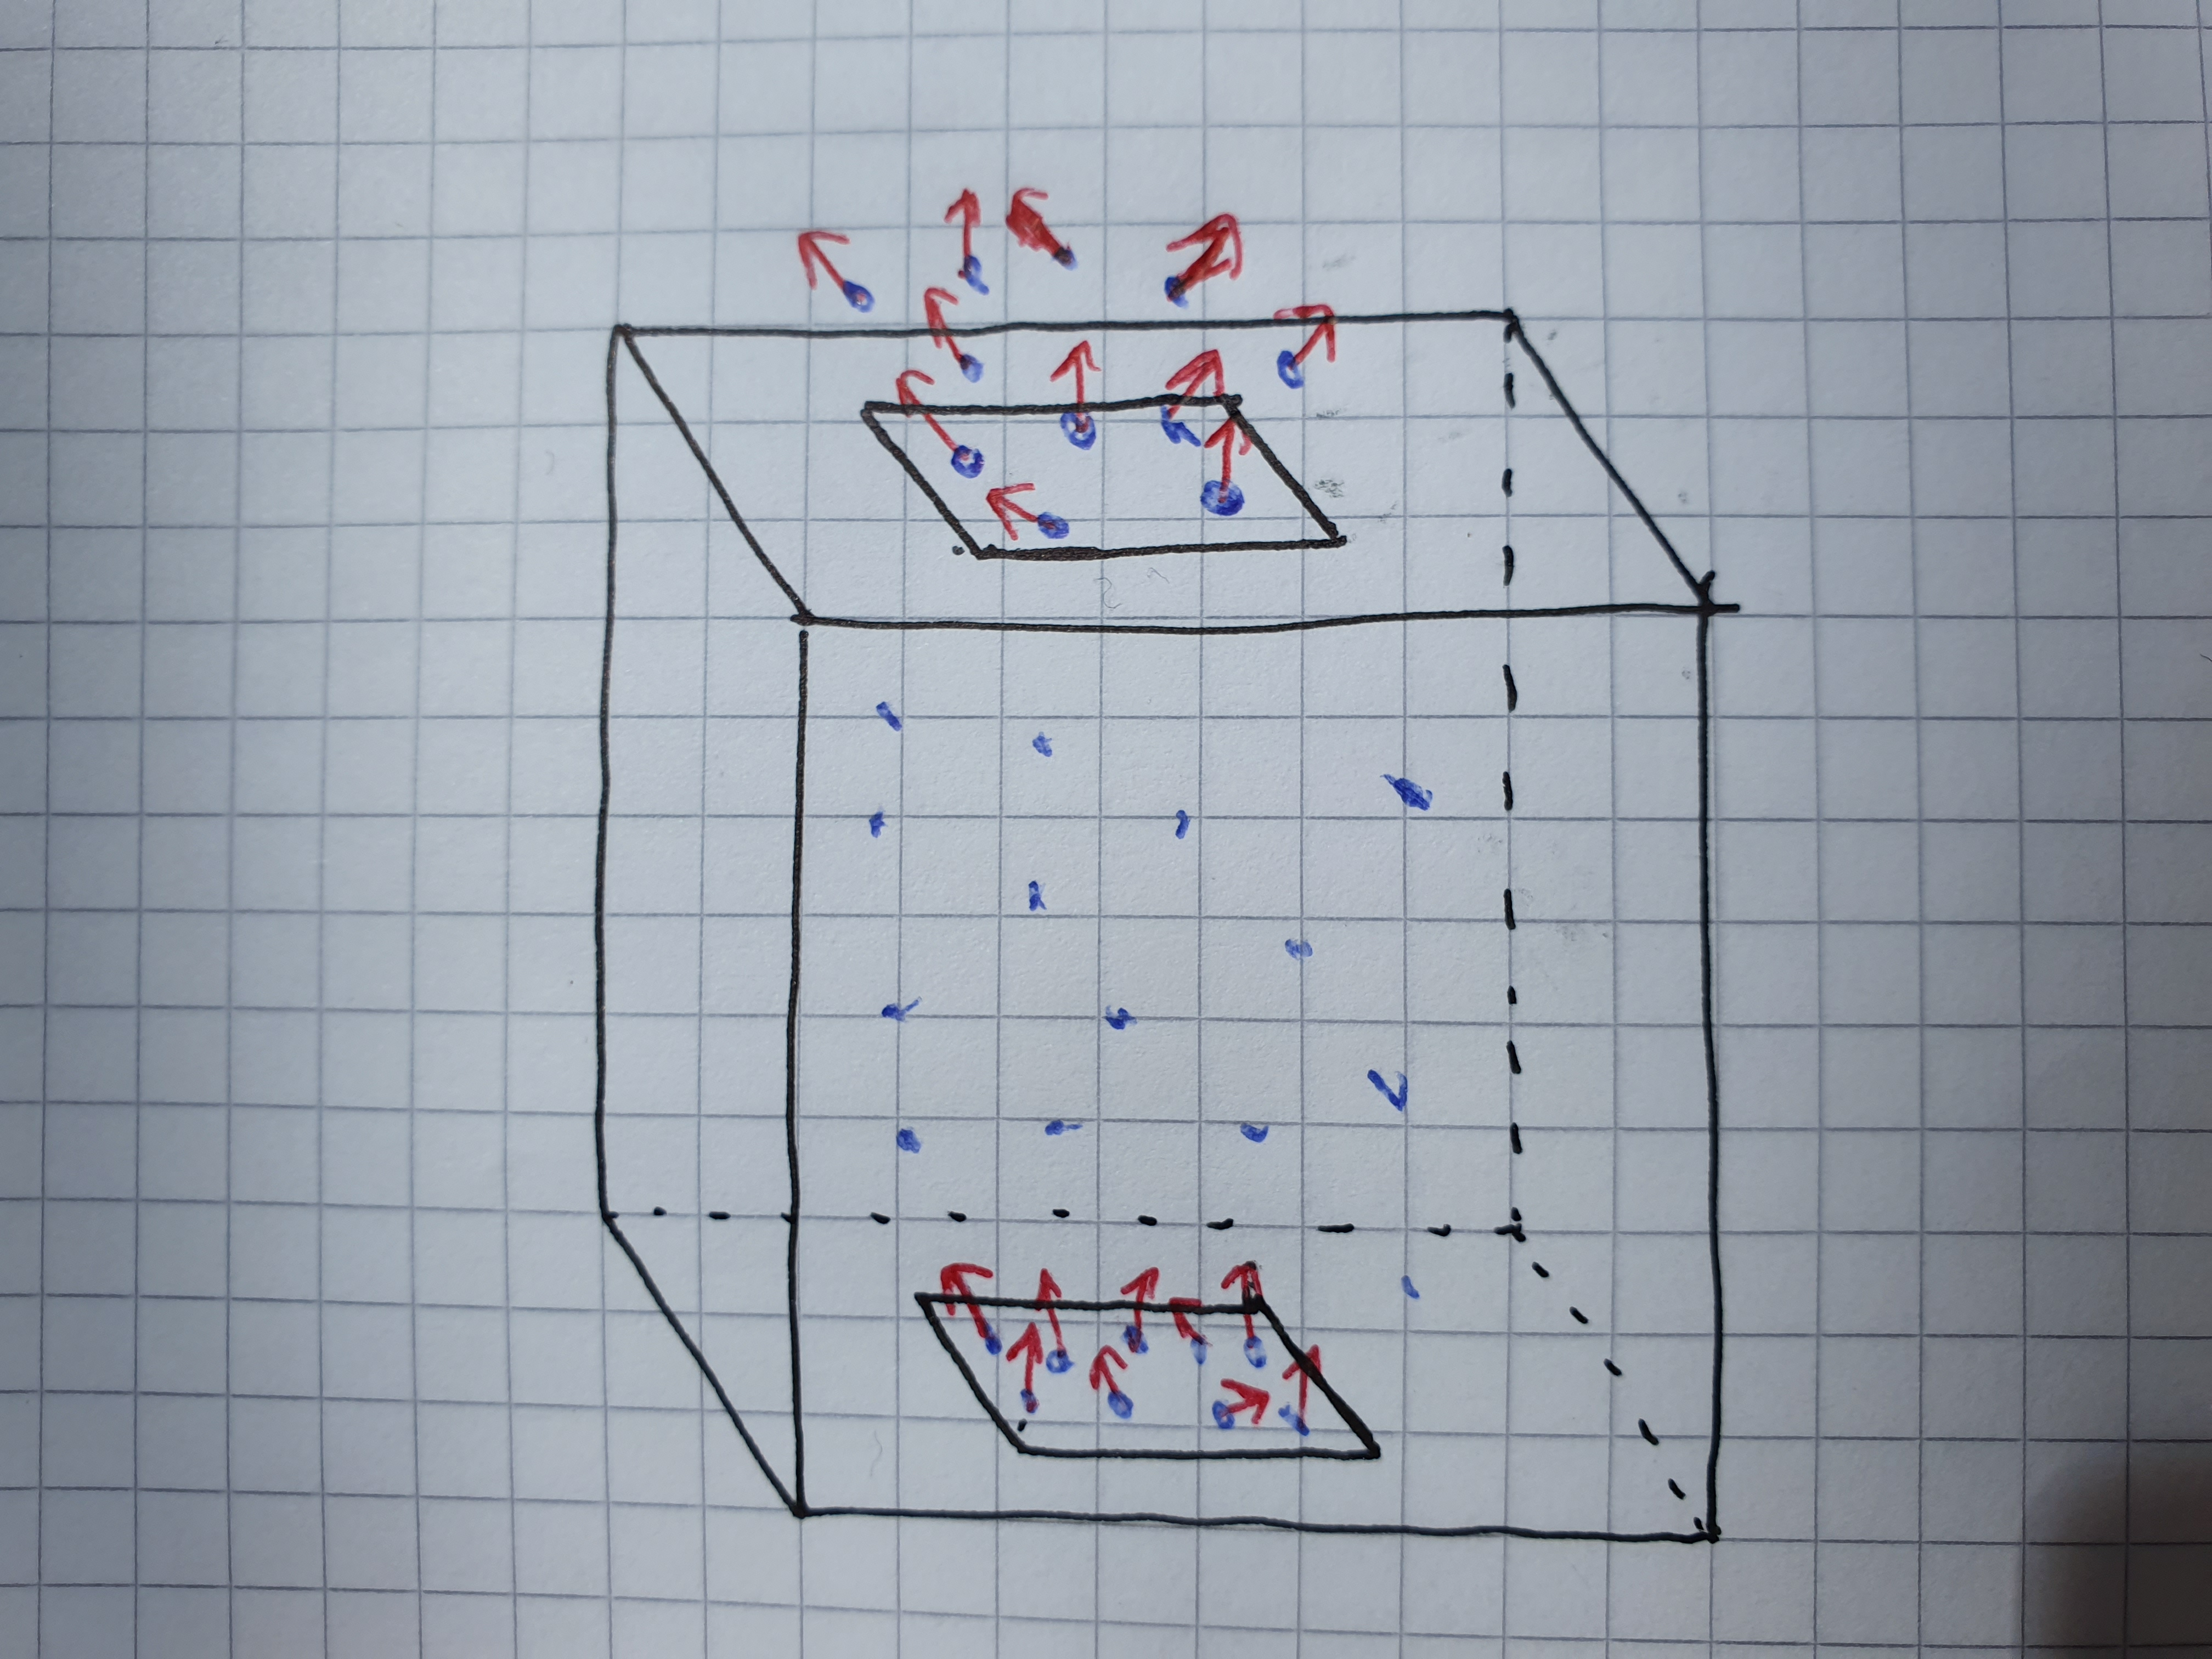
\includegraphics[angle=180, origin=c, width=0.5\linewidth]{boks_hull.jpg}
\caption{Denne figuren viser boksen med to kvadratiske hull. Hullene har sidelengder $L/2$. Partiklene kolliderer med veggene i boksen, og slipper etterhvert ut gjennom hullet i bunnen. Idet en partikkel slipper ut, kommer det en ny inn gjennom hullet på toppen. Ingen partikler slipper ut av boksen gjennom hullet på toppen. \label{fig:boks_hull}}
\end{figure}

Ved å registrere bevegelsesmengden til alle partiklene som slipper ut, kan vi nå beregne
 akselerasjonen som raketten får i løpet av simulasjonen. Vi ser bort fra gravitasjonskraften, da skal bevegelsesmengden til systemet som består av rakett om gassmolekyler være bevart. Det betyr at raketten vil få en økning i bevegelsesmengde som er like stor som, men motsatt rettet av, bevegelsesmengden til partiklene som slipper ut gjennom gulvet. Når vi måler bevegelsesmengden til partiklene som unnslipper, holder det å måle i den ene retningen som står normalt på veggen med hullet. Grunnen til dette er at hastigheten i de andre retningene er normalfordelt slik at bevegelsesmengden til forskjellige partikler vil utklikne hverandre i de andre retningene. Bevegelsesmengde er gitt ved
 \[
 \vec{p} = m \vec{v}
 \]
 der $m$ er masse og $\vec{v}$ er hastighet. Fartsøkningen til raketten i løpet av simulasjonen blir da
 \[
 \Delta v_{sim} = p/m
 \]
 der $p$ er den samlede bevegelsesmengden i én retning til partiklene som slipper ut i løpet av simulasjonen og $m$ er massen til raketten med satelitten, altså 1000kg.

Målet med prosjektet er å finne ut hvor stor motor og hvor mye drivstoff vi trenger for å
  akselerere raketten til planetens unnslipningshastighet i løpet av 20 minutter. Nå som vi vet hvor stor fartsøkning vi får fra én boks i løpet av én simulasjon $\Delta v_{sim}$, kan vi finne ut hvor mange bokser vi trenger for å få den nødvendige fartsøkningen i løpet av 20 minutter. Fartsøkningen vi får i løpet av ett sekund er $\Delta v = \frac{\Delta v_{sim}}{\Delta t}$, der $\Delta t$ er varigheten til simulasjonen. Vi kaller antall bokser vi behøver $m$. Farten vi skal oppnå er unnslipningshastigheten $v_{esc}$ til planeten. Vi vil at
  \[
  v_{esc} = 1200 m \Delta v
  \]
  siden fartsøkningen skal skje over 20 minutter, som tilsvarer 1200 sekunder, og får da at antall bokser vi trenger er
 \[
 m = \frac{v_{esc}}{1200 \Delta v} = \frac{v_{esc} * \Delta t}{1200 \Delta v_{sim}}
 \]

Massen til drivstoffet vi trenger for å nå denne hastigheten er simpelthen summen av massen
 til alle gassmolekylene som slipper ut av alle boksene våre i løpet av de 20 minuttene. Under simulasjonen teller vi antall partikler $n_{esc}$ som unnslipper én boks. Vi har at det totale antallet partikler som unnslipper alle boksene er
 \[
 N_{esc} = 1200 * m * n_{esc}
 \]
 Den samlede massen til alle partiklene som har forsvunnet blir da
 \[
 M_{esc} = m_{H2} * N_{esc}
 \]

Denne beregnede massen kan vi også sjekke mot en analytisk verdi. Ettersom vi antar at
 bevegelsesmengden til systemet som består av satelitten og gasspartiklene er bevart kan vi si at bevegelsesmengden som satelitten har når den har oppnådd unnslipningshastigheten skal være den samme som den samlede bevegelsesmengden til alle partiklene som har blitt skutt ut av boksene. Vi ser også bort fra massetapet til raketten. Vi kjenner den gjennomsnittlige farten $v$ til partiklene i gassen analytisk. Da kan vi også finne bevegelsesmengden i retningen som peker ut av boksen til én partikkel som unnslipper, se \citep{part1A}. Den er gitt ved
 \[
 p_{partikkel} = m_{H2}*v/\sqrt{3}
 \]
 Den samlede bevegelsesmengden til alle partiklene som unnslipper er da
 \[
 p_{partikler} = N_{esc} * p_{partikkel} = M_{esc} * v /\sqrt{3}
 \]
 Bevegelsesmengden som satelitten må ha for å ha oppnådd unnslipningshastigheten er gitt ved $p_{rakett} = M*v_{esc}$ der M er massen til satelitten. Setter vi $p_{rakett} = p_{partikler}$ kan vi løse denne for $M_{esc}$, som forteller hvor mye masse som må slippe ut for å gi oss den farten vi ønsker:
 \begin{equation}
   \label{eq:fuelmass}
   M_{esc} = \frac{M * v_{esc} * \sqrt{3}}{v}
 \end{equation}




\section{Resultater}

Vi kjører simuleringen med $N = 10^5$. Når vi sammenlikner hastighetene i x-, y- og z-
 retning etter initialiseringen med det analytiske uttrykket for normalfordeling\citep{part1A} får vi fordelingen i figur \ref{fig:boltzmann}.

\begin{figure}[htbp]
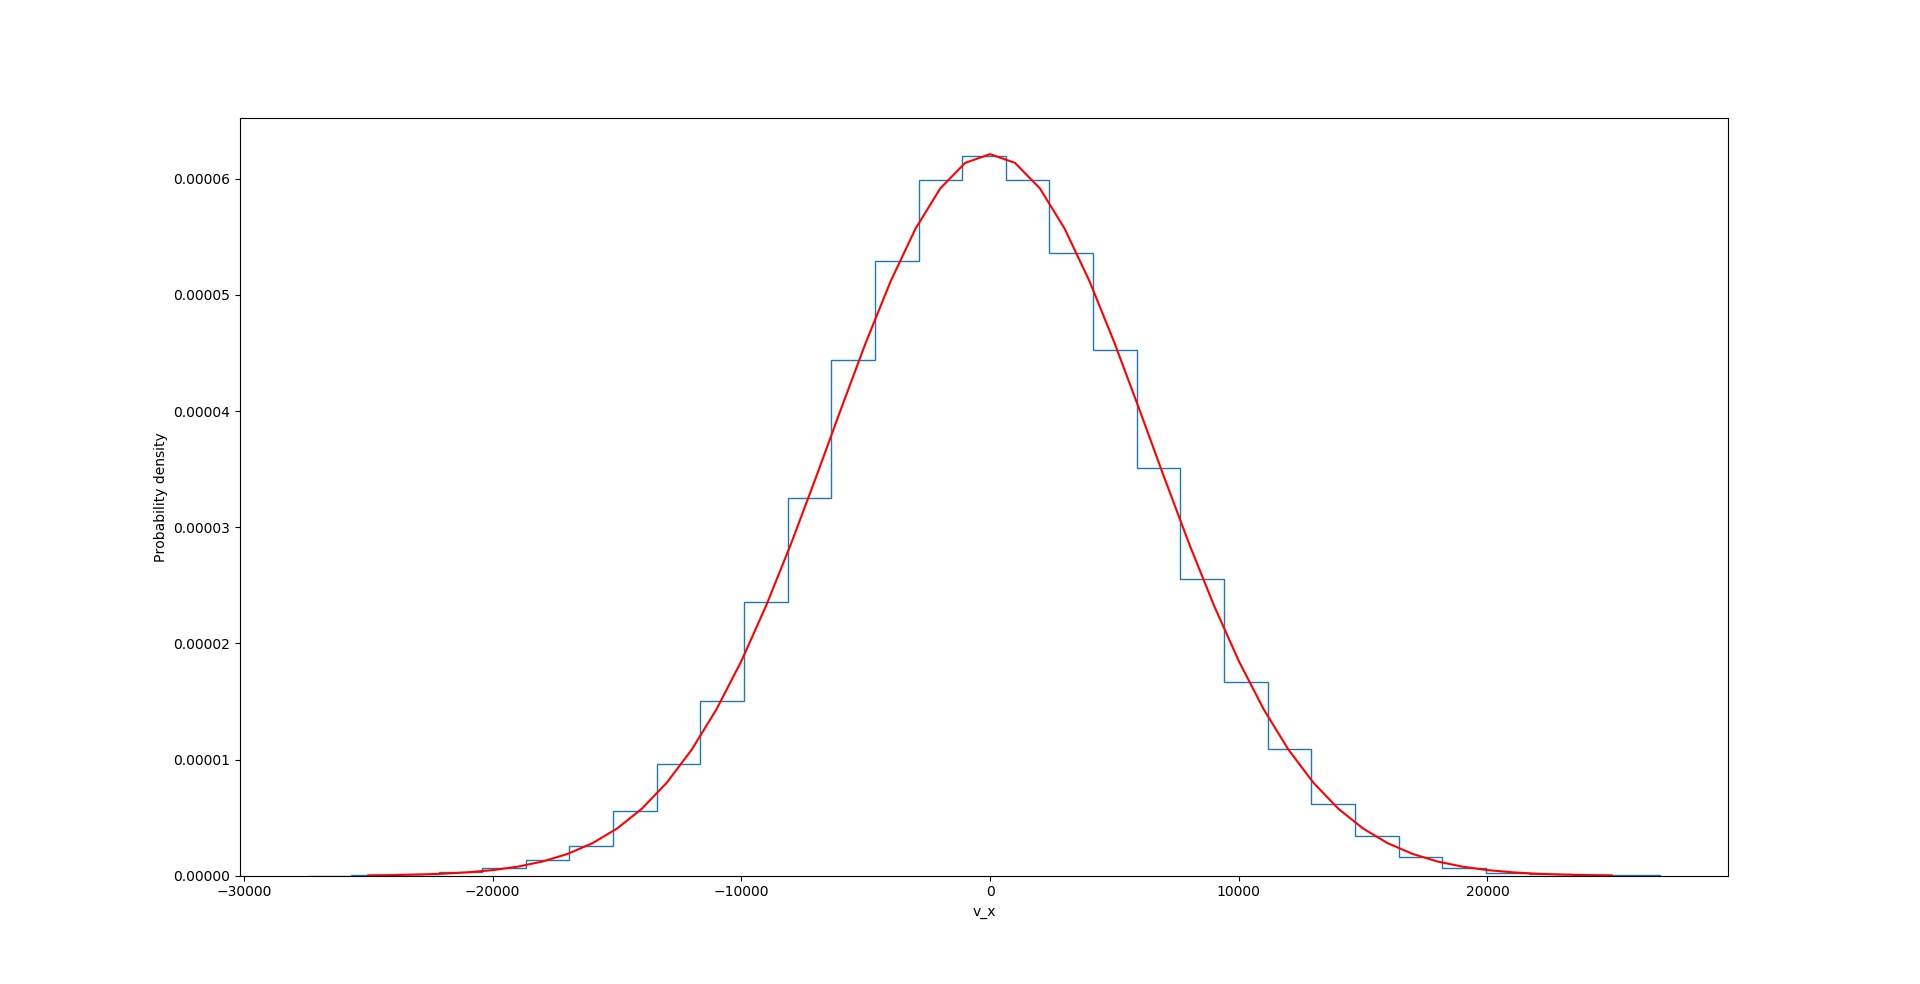
\includegraphics[width=\linewidth]{/home/vegard/Documents/v_x.jpg}
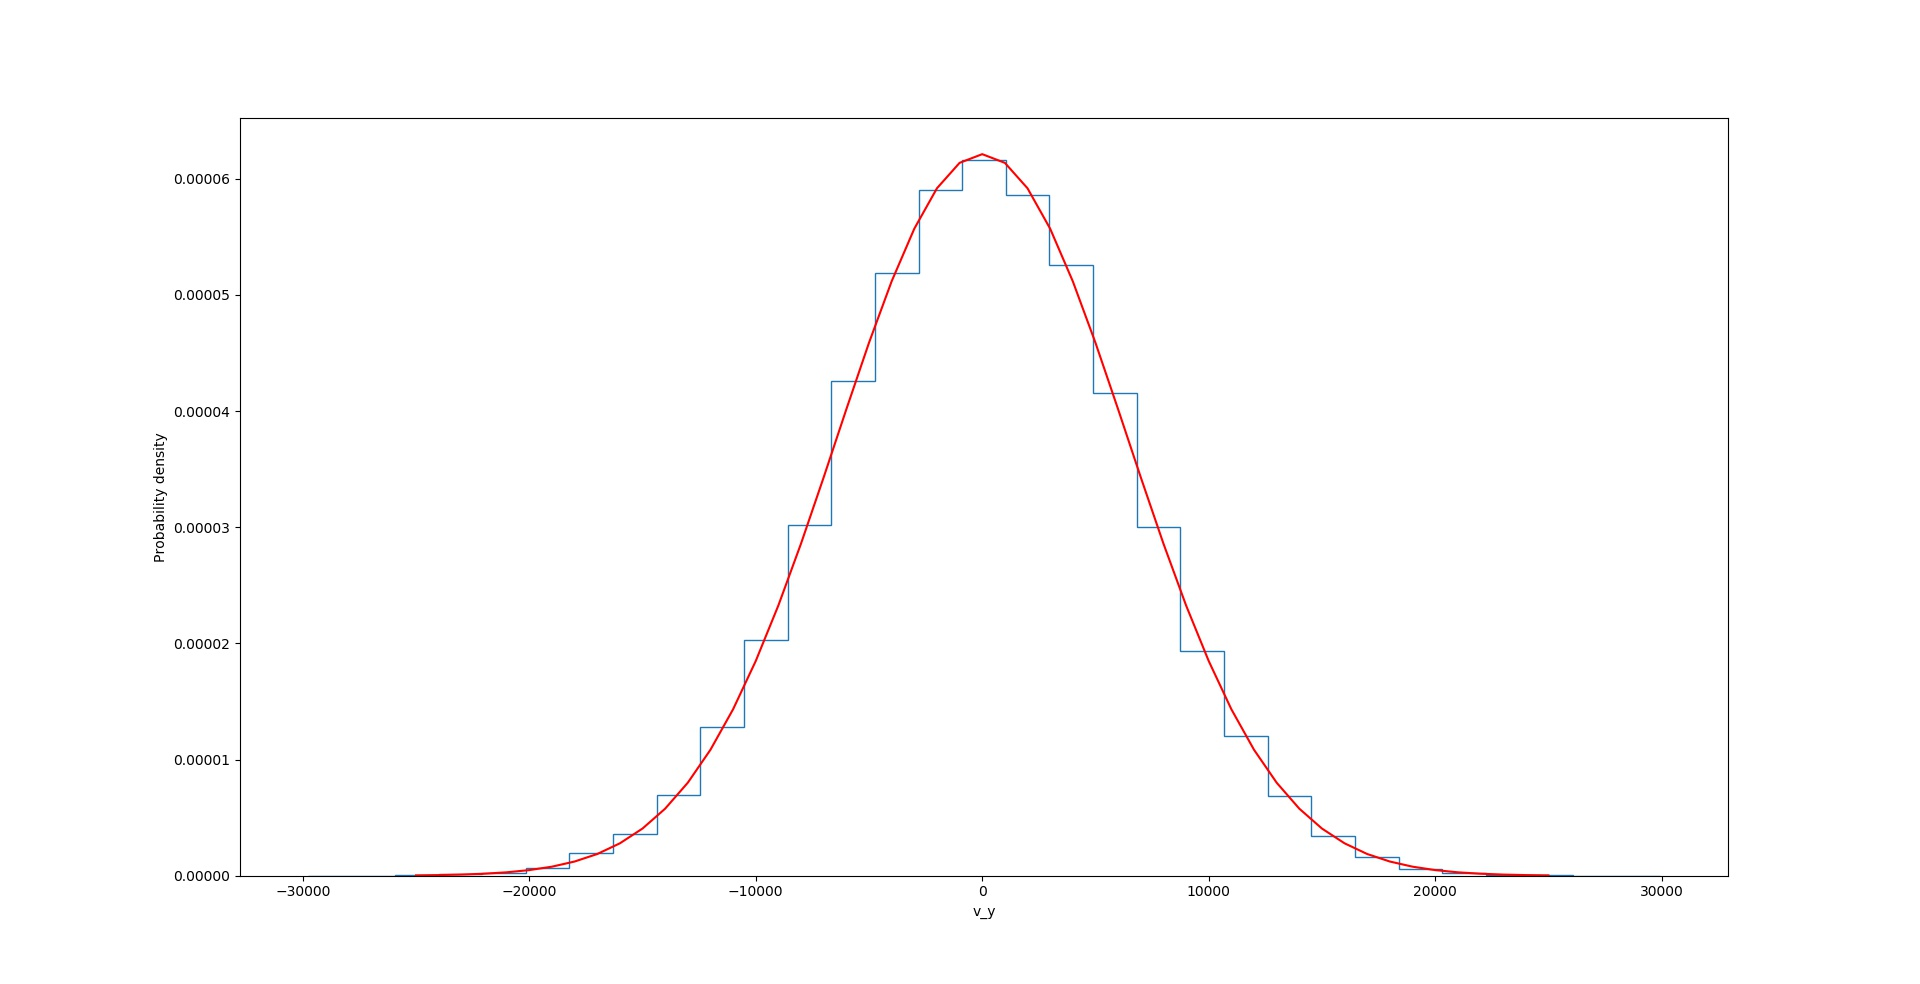
\includegraphics[width=\linewidth]{/home/vegard/Documents/v_y.jpg}
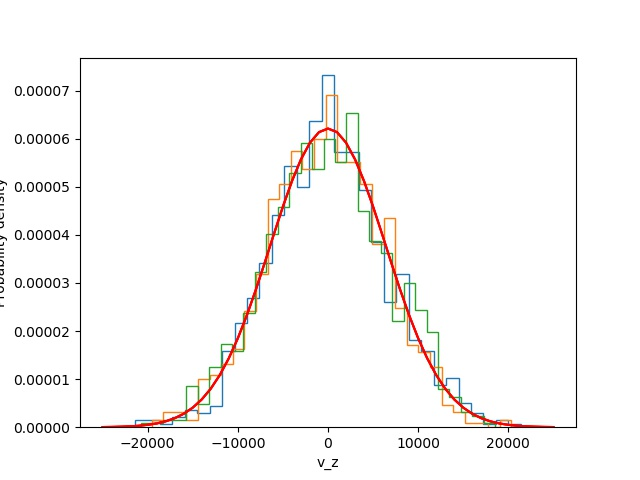
\includegraphics[width=\linewidth]{/home/vegard/Documents/v_z.jpg}
\caption{Histogram av hastighetskomponentene i x, y og z-retning tatt fra alle partiklene ved $t=0$. Den røde linjen viser Maxwell-Boltzmannfordelingen basert på temperaturen til disse partiklene.\label{fig:boltzmann}}
\end{figure}

Vedlagt er en tabell som viser resultatene av å kjøre simulasjonen med forskjellig antall
 partikler. Jeg ønsker å trekke fram et par resultater. Vi finner f.eks. at med 100 000 partikler i hver boks, trenger vi ca $6,0*10^12$ bokser for å nå unnslipningshastighet i løpet av 20 minutter. Legger vi alle disse boksene side om side, utgjør de et areal på rundt 0.0020$m^2$ eller 20$cm^2$. Det betyr at vi skal kunne akselerere raketten etter behovene våre med en motor hvis bunn er et kvadrat med sidekanter 4.5cm. Det største relative avviket mellom beregnet verdi og analytisk verdi jeg fikk i resultatene er for tap av drivstoff. Vi kommer noe nærmere med flere partikler, men med 100 000 partikler har vi fortsatt en realtiv feil på 26,9\%.


\section{Diskusjon}

Vi ser først og fremst tydelig at modellen virker til å stemme bedre med analytiske uttrykk
 når vi øker antall partikler. I de fleste tilfeller reduseres den relative feilen når vi øker antall partikler. Ved å sjekke gjennomsnittshastigheten og den gjennomsnittlige kinetiske energi til partiklene med det analytiske uttrykket \ref{eq:kinetic} ser vi at implementeringen av initialhastigheter var vellykket. Dette ser vi også av figur \ref{fig:boltzmann}.

Når vi sammenlikner det simulerte trykket mot det analytiske uttrykket \ref{eq:fuelmass},
 får vi en relativ feil på mellom 1.3\% og 2.3\%. Den relative feilen er veldig lik for 1 000 og 10 000 partikler, men betraktelig lavere for 100 000 partikler. Det er naturlig at vi får en feilmargin når vi beregner trykket på grunn av modellen jeg har valgt å bruke for å snu partiklene når de kolliderer med veggene. Vi ser at det beregnede trykket alltid er høyere enn det analytiske trykket. Det kan tyde på at de fleste partiklene blir snudd før de egentlig treffer veggen, altså at algoritmen ikke virker helt som ønsket. Vi kunne prøvd å korrigere dette ved å flytte på buffersonen med en prøv-og-feil-tilnærming, men jeg mener at resultatet vi har er akseptabelt.

Når det gjelder tap av drivstoff, er det tydelig at vi har et stort avvik mellom beregnet
 og analytisk verdi. Hvor denne feilen kommer fra er ikke tydelig. I det analytiske uttrykket regner vi med konstant trykk og temperatur. I simuleringen har vi også hele tiden konstant temperatur (kinetisk energi), men hva som skjer med trykkfordelingen når vi tar ut partikler gjennom et hull i den ene siden og fyller på med partikler gjennom et hull i den andre siden, er kanskje ikke helt trivielt. Det kan tenkes at noe av avviket kan forklares ved å studere dette. Det er selvfølgelig også mulig at det er en feil i koden som gjør at resultatet blir feil.

Når det gjelder anvendelse av de resultatene vi har funnet, må vi huske på alle
 forenklingene vi har gjort underveis. For det første ser vi bort fra tyngdekraften under akselerasjonen, noe som åpenbart ikke er reelt. I virkeligheten vil gravitasjonskraften fra jorda gjøre at vi trenger mye mer drivstoff, og flere bokser, for å komme opp i unnslipningshastigheten. Unnslipningshastigheten i det punktet raketten befinner seg i vil også endre seg etter hvert som den beveger seg lenger bort fra planeten fordi den er avhengig av massen til planeten og avstanden til planetens massesenter\citep{part1A}. I tillegg har vi ignorert at raketten vil tape masse etterhvert som gasspartiklene forsvinner ut på undersiden. Vi antar at trykket i boksene er konstant, noe som gir oss konstant framdriftskraft. Når massen da blir mindre, betyr det at akselerasjonen blir større og større.

Vi må også forvente noen avvik fra virkeligheten på grunn av forenklingene vi har gjort
 knyttet til gassen i beholderne. Vi ser bort fra all interaksjon mellom partiklene, det eneste som påvirker bevegelsen til gassmolekylene er når de kolliderer med veggene i boksen. 


\section{Konklusjon}

ABSTRACT OG KONKLUSJON er ikke ferdig.

Vi har laget en meget forenklet kode for stjernedannelse. Metoden har klare begrensninger da vi ikke tar hensyn til interaksjon mellom partiklene som trengs for å inkludere effektene av f.eks. gasstrykk. Vi tar heller ikke hensyn til strålingen som oppstår, i tillegg til at vi for å lage koden raskere deler gass-skya opp i et begrenset antall kuleskall som gjør at simuleringen bryter sammen når mange partikler har fallt inn til det innerste skallet.


\section{Vedlegg}

\begin{figure}[p]
  \begin{tabular}{||c c c c||}
  \hline
  No. of particles & 1 000 & 10 000 & 100 000 \\ [0.5ex]
  \hline\hline
  Kinetic energy: &  &  &  \\
  \hline
  Computed mean, J & $2.08855*10^{-19}$ & $2.08915*10^{-19}$ & $2.07298*10^{-19}$ \\
  \hline
  Analytical mean, J & $2.0715*10^{-19}$ & $2.0715*10^{-19}$ & $2.0715*10^{-19}$ \\
  \hline
  Relative error & 0.82\% & 0.85\% & 0.07\% \\

  \hline\hline
  Velocity: &  &  &  \\
  \hline
  Computed mean, m/s & 10321.63 & 10301.20 & 10258.07 \\
  \hline
  Analytical mean, m/s & 10249.67 & 10249.67 & 10249.67 \\
  \hline
  Relative error & 0.70\% & 0.50\% & 0.08\% \\

  \hline\hline
  Pressure test (closed box):  &  &  &  \\
  \hline
  Hits & 2579 & 26187 & 260799 \\
  \hline
  Escaped & 0 & 0 & 82 \\
  \hline
  Computed P, Pa & 141.16 & 1412.25 & 13995.02 \\
  \hline
  Analytical P, Pa & 138.10 & 1381.00 & 13810.00 \\
  \hline
  Relative error & 2.21\% & 2.26\% & 1.34\% \\

  \hline\hline
  Rocket simulation: &  &  &  \\
  \hline
  Hits & 2184 & 21888 & 217706 \\
  \hline
  Escaped & 732 & 7938 & 76666 \\
  \hline
  Momentum gain, kg m/s & $2.0967*10^{-20}$ & $2.16334*10^{-19}$ & $2.07807*10^{-18}$ \\
  \hline
  No. of boxes & $5.913*10^{14}$ & $5.730*10^{13}$ & $5.966*10^{12}$ \\
  \hline
  Fuel loss, kg & 1738.52 & 1827.22 & 1837.16 \\
  \hline
  Analytical fuel loss, kg & 2513.86 & 2513.86 & 2513.86 \\ [1ex]
  \hline
 \end{tabular}
\caption{Tabell som viser resultatene av å kjøre simulasjonen med forskjellig antall partikler. Temperaturen er hele tiden 10 000K.\label{fig:tabell}}
\end{figure}





\begin{thebibliography}{}
\bibitem[Hansen (2017)]{part1A} Hansen, F. K.,  2017, Forelesningsnotat 1A i kurset AST2000


\end{thebibliography}



\end{document}
